\documentclass[handout]{beamer}

\usepackage{fontspec} 
\useoutertheme{lsp}

\usepackage{lsptitle}
\usepackage{booktabs}
\def\two@digits#1{\ifnum#1<10 0\fi\number#1}
\def\mytoday{\two@digits{\number\day}.\two@digits{\number\month}.\number\year}


\usepackage{xspace,multicol}
\newcommand{\latex}{\LaTeX\xspace}
\usepackage{tikz}


\newcounter{lastpagemainpart}
\footnotesep0pt
\renewcommand{\footnoterule}{}
\usefootnotetemplate{
  \noindent
  \insertfootnotemark\insertfootnotetext}

\let\beamerfn=\footnote
\renewcommand{\footnote}[1]{\%
\let\oldfnsize=\footnotesize\%
\let\footnotesize=\tiny\%
\beamerfn<\thebeamerpauses->{#1}\%
\let\footnotesize=\oldfnsize}


\date{\today}

\usepackage{eurosym}  
 
\renewcommand{\centerline}[1]{\hfill#1\hfill\hfill\mbox{}}


\title{\mbox{Community Proofreading}\\
\mbox{Zielstellung, Implementation, Evaluation}
\institute{Language Science Press}
\author[LangSci]{Sebastian Nordhoff}



\begin{document}
\lspbeamertitle

\section{OA $\to$ Open Publishing}

Um eine widerstandsfähige und tragfähige wissenschaftsgeführte OA-Publikationsplattform wie z.B. Language Science Press aufzubauen und zu betreiben, ist die Einbindung der Community zentral. Nur wenn die Community die Verlagsplattform als "ihre" Plattform annimmt und ihr eine wesentliche Position in der Publikationslandschaft zuschreibt, kann solch eine Plattform längerfristig Bestand haben.
Eine neuartige Form des Community-Buildings ist das sogenannte Community-Proofreading. Hierbei wird statt eines klassichen Korrektorats die formale Qualitätssicherung an die Leser "crowdgesourct". Einzelne Forscher*innen lesen und korrigieren die Vorabversion je eines Kapitel eines neuen Buches. Hierzu wird die Plattform PaperHive verwendet. Westedt (2018) hat eine erste qualitative Analyse dieses Vorgehens vorgenommen. Ihre Arbeit wird in diesem Vortrag ergänzt um eine quantitative Analyse von über 43.000 Kommentaren von 228 verschiedenen Accounts in insgesamt 52 Büchern, die bei Language Science Press Community-Proofreading durchlaufen haben.
Hierbei zeigt sich, dass diese Kommentare (unter CC-BY-Lizenz) eine eigene Textsorte darstellen, die Einblicke in psychologische Prozesse beim Lesen und Korrigieren ermöglicht. Die Verwendung einer interoperablen und vernetzten Plattform wie PaperHive mit einer offenen API eröffnet hier ganz neue Nachnutzungsmöglichkeiten von Daten, die im Publikationsprozess bisher eher als Nebenprodukt angesehen wurden. Durch den Verzicht auf eine Gatekeeper-Funktion des Verlages können diese Daten der Wissenschaft zur Verfügung gestellt werden.
In einer weiteren Analyse wird gezeigt, dass die Autorenbindung durch Community-Proofreading gestärkt wird und dass zukünftige Autoren schon während des Studiums an die "community-eigene" Plattform herangeführt werden.
Die strikte Trennung der Rollen von Autor*in, Leser*in und Gutachter*in verschwimmt in kollaborativen Prozessen, wie wir sie bei Open-Access-Publikationen finden. Community-Proofreading bildet die stärkere Einbindung der Leserin in den Publikationsprozess ab und leistet so einen wichtigen Beitrag zu community-based/scholar-led Publishing.

\frame{
\frametitle{Open Publishing}
%   \includegraphics[height=.6\textheight]{./path/to/graphicsfile}
  \begin{itemize}
    \item im Open Access geht es meistens um Zugang, d.h. ums Lesen
    \item Open Publishing geht darüber hinaus: 
    \begin{itemize}
      \item Open source platforms 
      \item Open formats 
      \item Open protocols
      \item Open bookkeeping 
      \item Open peer review
      \item Community proofreading
    \end{itemize}    
  \end{itemize}
}

\section{Community}
\frame{
\frametitle{Bibliodiversität (Pierre Mounier)}
%   \includegraphics[height=.6\textheight]{./path/to/graphicsfile}
  \begin{itemize}
    \item Forschende nehmen je nach Uhrzeit ganz verschiedene Rollen ein
    \begin{itemize}
      \item Autor, Gutachterin, Leserin
    \end{itemize}
    \item je jünger desto Leser
    \item je älter desto Gutachter
    \item komplexes Ökosystem
    \item Integration aller Ebenen im community-based Publishing
  \end{itemize}
}


\section{Community proofreading}
\frame{
\frametitle{Traditionalles Lektorat/Korrektorat}
%   \includegraphics[height=.6\textheight]{./path/to/graphicsfile}
  \begin{itemize}
    \item eingekaufte Dienstleistung
    \item 1 Person
    \item spezialisiert in Stil und Richtlinien
    \item fachlicher Hintergrund möglich aber nicht zwingend 
    \item normalerweise kein Spezialwissen in spezifischen Teilgebieten der Linguistik
  \end{itemize}
}

\frame{
\frametitle{Community proofreading}
%   \includegraphics[height=.6\textheight]{./path/to/graphicsfile}
  \begin{itemize}
    \item Crowdsourcing
    \item freiwillig
    \item viele Korrektoren, häufig jünger
    \item sehr häufig Spezialisten im Teilgebiet
    \item intrinsisches Interesse
    \item relativ gesehen geringere Expertise in Stilistik und Richtlinien
  \end{itemize}
}

\frame{
\frametitle{Language Science Press}
%   \includegraphics[height=.6\textheight]{./path/to/graphicsfile}
  \begin{itemize}
    \item  Open-Access-Verlag in der Sprachwissenschaft
    \item 100+ Bücher seit 2014 
    \item 350 Community Proofreader
  \end{itemize}
}

\frame{
\frametitle{Katalog}
  
\includegraphics[height=\textheight]{catalog.png}
}

\frame{
\frametitle{Workflow}
  \begin{itemize}
    \item Proofreading Queue: neuer Titel alle 2 Wochen
    \item Titel wird montags angekündigt
    \item Interessierte können sich für ein Kapitel melden
    \item Kapitel werden mittwochs zugewiesen
    \item Dauer: 4 Wochen
    \item Software: Paperhive
  \end{itemize}
}

\frame{
\frametitle{Paperhive}
  
\includegraphics[width=\textwidth]{paperhive.png}
}

\section{Study}
\frame{
\frametitle{Westedt (2018)}
\begin{itemize}
  \item 
Westedt hat eine Stichprobe von Kapiteln hinsichtlich der Kommentare analysiert:
\end{itemize}

\centering 
\begin{tabular}{lr}
Category & Percentage\\
\midrule 
Stil&21.00\\
Lexik&20.73\\
Zeichensetzung&11.81\\
Grammatik&11.55\\
Referenzen&9.71\\
Syntax&7.80\\
Rechtschreibung&7.30\\
\textbf{Inhalt}&\textbf{6.56}\\
Verschiedenes&3.41\\
\end{tabular}
}


\frame{
\frametitle{Quantitative Analyse}
%   \includegraphics[height=.6\textheight]{./path/to/graphicsfile}
  \begin{itemize}
    \item  52 Bücher (2016--2018)
    \item Paperhive-Kommentare wurden per API in eine Datenbank überführt
    \item 19\,004 Seiten 
    \item 43\,370 Kommentare
    \item data on \url{https://doi.org/10.5281/zenodo.3063004}
  \end{itemize}
}

\section{Statistik}
\frame{
\frametitle{Länge der Bücher}
  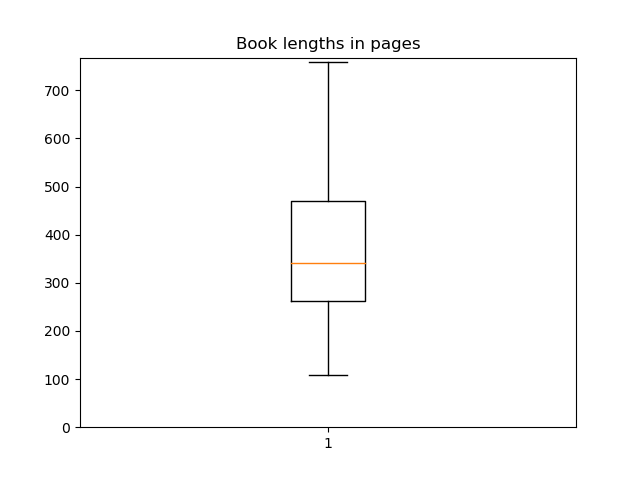
\includegraphics[height=\textheight]{booklengths.png}
}

\frame{
\frametitle{Menge Kommentare}
  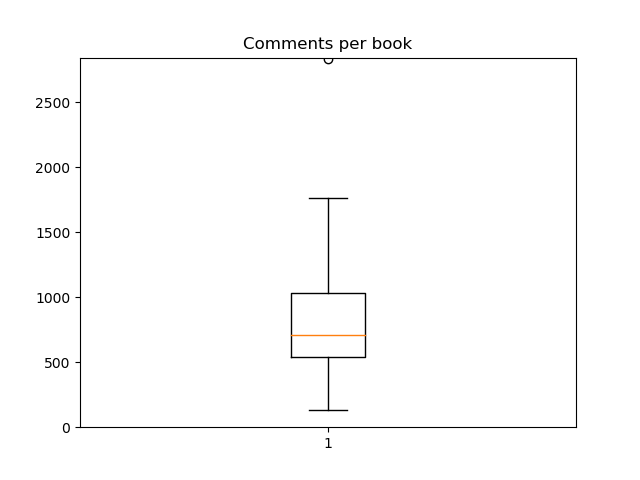
\includegraphics[height=.6\textheight]{commentsperbook.png}
  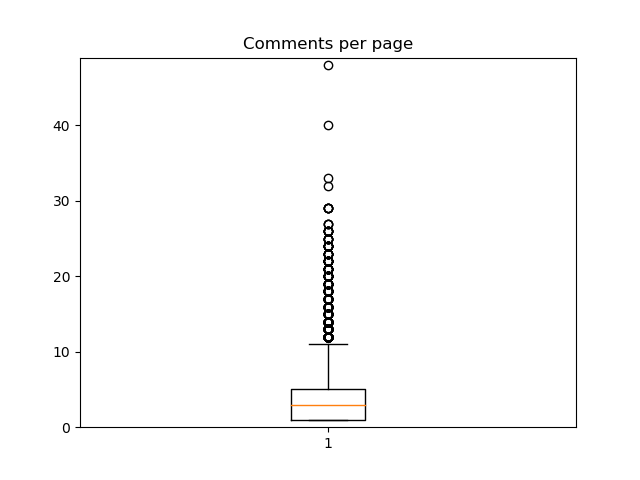
\includegraphics[height=.6\textheight]{commentsperpage.png}
  Die höchste Anzahl Kommentare auf einer Seite findet sich auf Seite 122 von  \textit{Theory and description in African Linguistics} (48 Kommentare).
}

\frame{
\frametitle{Proofreader}
  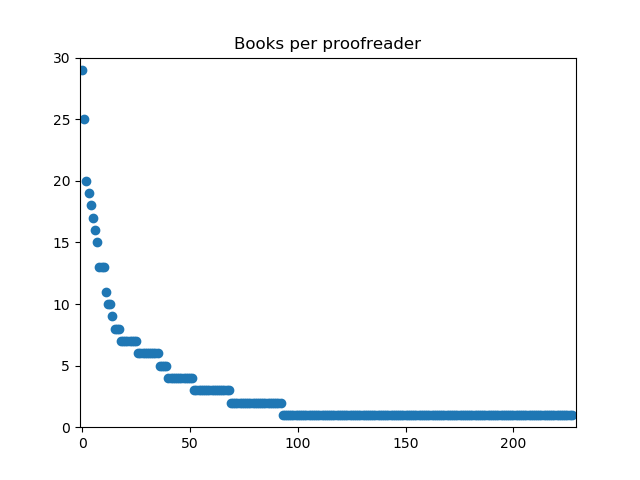
\includegraphics[height=.6\textheight]{booksperproofreader_p.png}
  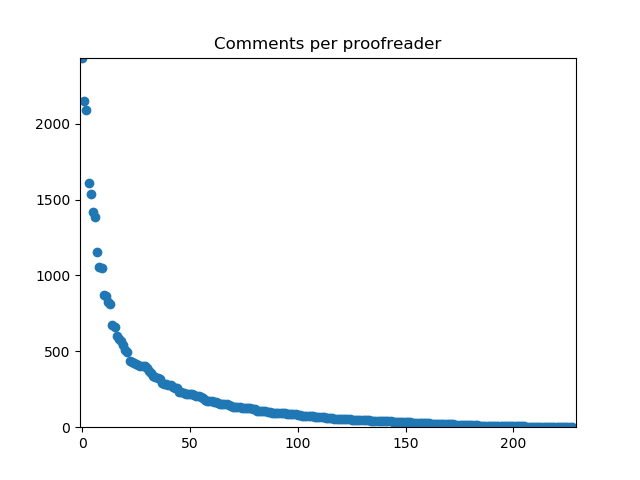
\includegraphics[height=.6\textheight]{commentsperproofreader_p.png}
228 verschiedene Accounts haben bisher am Community Proofreading teilgenommen. 
}

\frame{
\frametitle{Proofreader pro Buch}
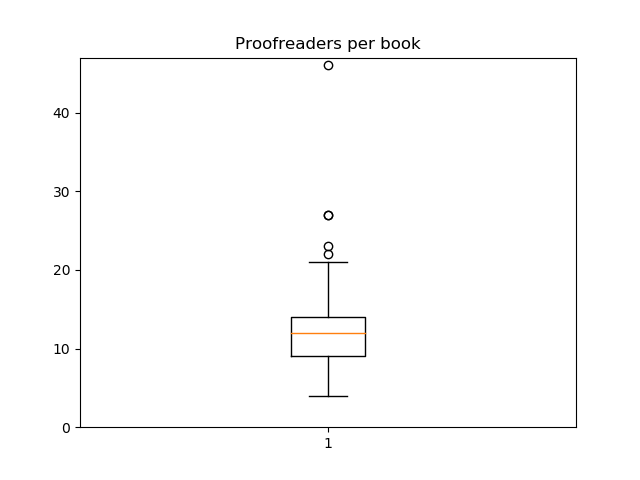
\includegraphics[height=\textheight]{proofreadersperbook.png}
  }

\frame{
\frametitle{Textanalyse der Kommentare}
  
\includegraphics[width=\textwidth]{commenttitlebody.png}
  \begin{itemize}
    \item  Kommentare auf PaperHive haben einen Titel (<40 Zeichen)
    \item zusätzliche Ausführungen in Freitextfeld optional möglich. 
  \end{itemize}
}

\frame{
\frametitle{Title length and body length}
  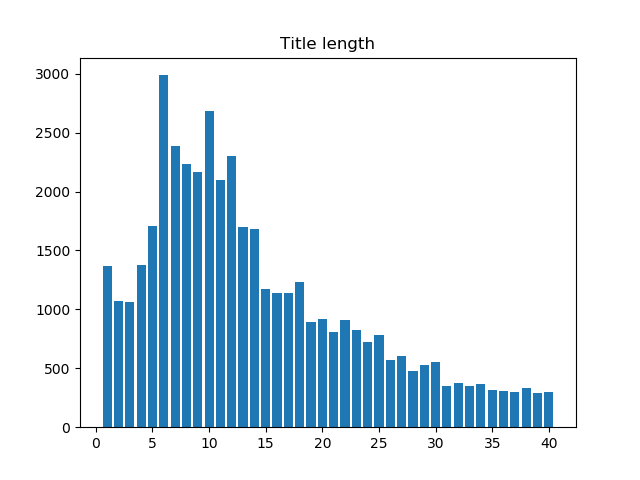
\includegraphics[height=.6\textheight]{titlelength_b.png}
  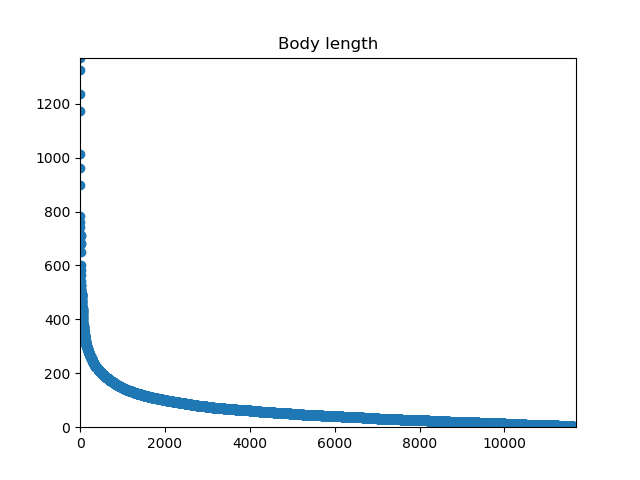
\includegraphics[height=.6\textheight]{bodylength_p.png}
}

\section{Hypothesen}
\subsection{Typologie}
\frame{
\frametitle{Hypothesen zu Proofreadern}
%   \includegraphics[height=.6\textheight]{./path/to/graphicsfile}
  \begin{enumerate}
    \item \textbf{Proofreader fallen in zwei Klassen: Typ 1 konzentriert sich auf kleine Details; Typ 2 sieht das Werk als Ganzes}
    \item \textbf{Kommentare werden gegen Ende des Kapitels kürzer (Ermüdung, Verweise auf vorher Gesagtes)}
  \end{enumerate}
}
 
\frame{
\frametitle{Hypothese 1:\\ 2 Klassen}
%   \includegraphics[height=.6\textheight]{./path/to/graphicsfile}
  \begin{itemize}
    \item  
Typ 1: viele Kommentare, dafür kurz (``comma missing'')
    \item 
    Typ 2: wenige Kommentare, dafür ausführlicher
  \end{itemize}
} 

\frame{
\frametitle{Berechnung}
%   \includegraphics[height=.6\textheight]{./path/to/graphicsfile}
  \begin{itemize}
    \item Für jedes Buch
    \begin{itemize}
      \item 
    ordne alle Teilnehmer nach Menge an Kommentaren
    \item ordne alle Teilnehmer nach durchschnittlicher Kommentarlänge
    \item trage beide Rangordnungen gegeneinander ab
    \end{itemize}
  \end{itemize}
}

\frame{
\frametitle{Beispielplot\\ for Hypothese 1}
  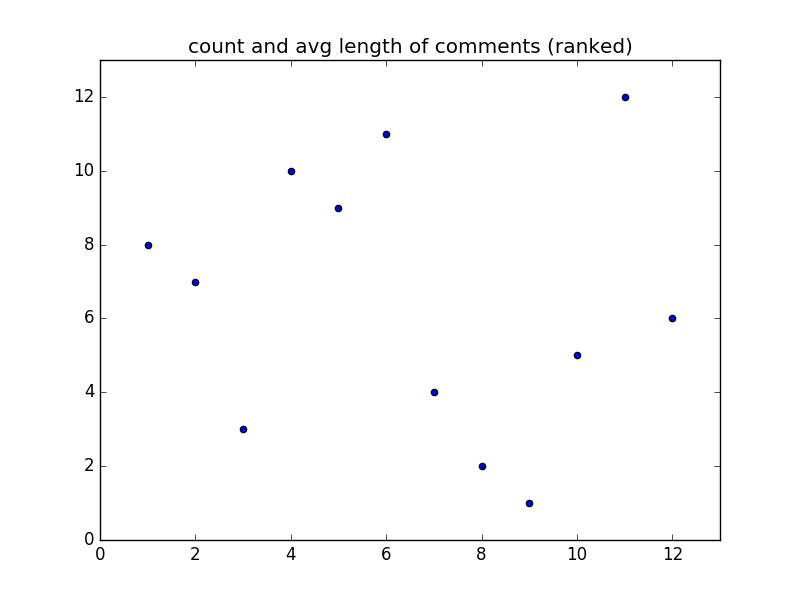
\includegraphics[height=.6\textheight]{allscatterx.png}
\begin{itemize}
  \item 12 Teilnehmer
  \item Rangfolge wird durch Punkte angegeben. 
  \begin{itemize}
    \item e.g. \#3 in Menge ist auch \#3 in Durchschnittslänge, aber \#1 entspricht \#8
  \end{itemize}
  \item Daten eines Buches offensichtlich nicht ausreichend.
\end{itemize}

  }

\frame{
\frametitle{Kombination aller Bücher}
  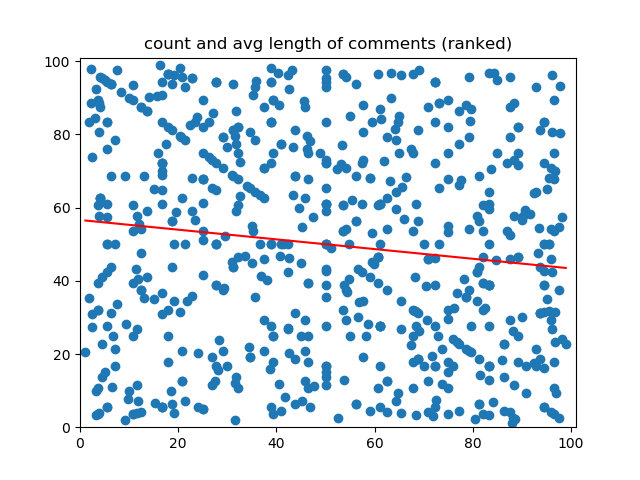
\includegraphics[height=.6\textheight]{allscatter.png}
  \begin{itemize}
    \item Ränge auf Perzentile normalisiert
    \item Rote Linie gibt best fit an
    \item in der Tat eine schwache negative Korrelation
  \end{itemize}
}
\frame{
\frametitle{Ergebnis Hypothese \#1}
%   \includegraphics[height=.6\textheight]{./path/to/graphicsfile}
  \begin{itemize}
    \item Hypothese \#1 bestätigt
    \begin{itemize}
      \item Proofreader mit mehr Kommentaren haben kürzere Kommentare
      \item Proofreaders with längeren Kommentaren haben weniger Kommentare
    \end{itemize}
  \end{itemize}
}


\subsection{Proofreader fatigue}
\frame{
\frametitle{Hypothesis \#2:\\ proofreader fatigue}
%   \includegraphics[height=.6\textheight]{./path/to/graphicsfile}
\textbf{Hypothesis 2 : Proofreading will diminish as the proofreader moves along. Comments will become shorter due to fatigue, i.e. average comment length will go down due to repetition of previous remarks as ``see above''.}
}

\frame{
\frametitle{\mbox{Computation for Hypothesis \#2}}
%   \includegraphics[height=.6\textheight]{./path/to/graphicsfile}
  \begin{itemize}
    \item for every book \\
     ~for every proofreader\\ 
       ~~for every comment
        \begin{itemize}
          \item compute relative length (e.g. 0.67 of the average)
          \item compute relative position (front, middle, back)
          \item store the tuple (relative position, relative length)
          \item A dot at (0.5, 5) means that there was a comment in the middle of the relevant stretch whose length was 5 times the average comment length. 
        \end{itemize}
\item the relative position can be pegged to the linear order of comments, or to the pages
    \end{itemize}
}

\frame{
\frametitle{Plot for Hypothesis \#2\\ based on linear order }
  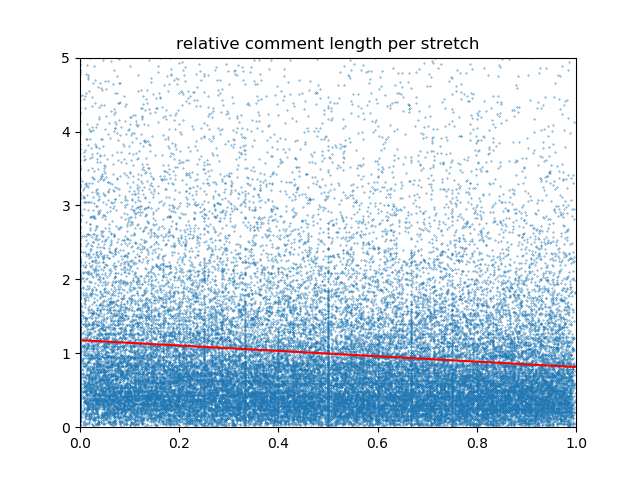
\includegraphics[height=\textheight]{stretches.png}
}

\frame{
\frametitle{Plot for Hypothesis \#2\\ based on page position }
  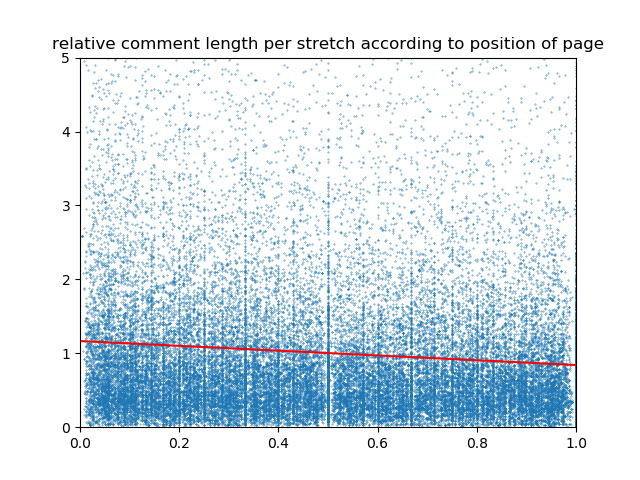
\includegraphics[height=\textheight]{stretchespages.png}
}

\frame{
\frametitle{Results for Hypothesis \#2\\ ``proofreader fatigue''}
%   \includegraphics[height=.6\textheight]{./path/to/graphicsfile}
  \begin{itemize}
    \item  Hypothesis is confirmed 
    \begin{itemize}
      \item the later in the document a comment is, the shorter it will be 
      \item the first comment will be about 110\% of the average, while the last one will be 90\% of the average.
      \item effect not very strong,  but discernible
    \end{itemize}
  \end{itemize}
}

\section{Discussion}
\frame{
\frametitle{Discussion}
%   \includegraphics[height=.6\textheight]{./path/to/graphicsfile}
  \begin{itemize}
    \item  Main aim: methodological
    \item Proofreading comments are a by-product of open publishing 
    \begin{itemize}
      \item In traditional publishing models, these data would not be available
    \end{itemize}
    \item Once the documents, processes, and formats are opened up, novel research questions can emerge which would not have been possible under a closed setup.  
    \item Implications for psychology of reading for instance.
  \end{itemize}
}

\section{The ecosystem}
\frame{
\frametitle{Do researchers take on\\ different roles? }
%   \includegraphics[height=.6\textheight]{./path/to/graphicsfile}
  \begin{itemize}
    \item  There are 908 people with the role ``author'' at LangSci Press 
    \item There are 228 proofreaders 
    \item 27 researchers have taken up both roles
    \begin{itemize}
      \item 16 started as authors, and became proofreaders later 
      \item 11 started as proofreaders, and became authors later
      \item Movement between the author pool and the proofreader pool in both directions. 
    \end{itemize}
  \end{itemize}
}

  
\section{Conclusions}
\frame{
\frametitle{Conclusions}
%   \includegraphics[height=.6\textheight]{./path/to/graphicsfile}
  \begin{itemize}
    \item  
Community proofreading is a novel way of engaging the community
    \item 
only possible for Open Access publications 
\item 
workable implementation with 50+ books and 200+ researchers
\item 
can compare to traditional proofreading 
\item 
by-product data can be used for novel research questions
\begin{itemize}
  \item proofreader typology 
  \item proofreader fatigue
\end{itemize}
\item flow back and forth between the group of authors and the group of proofreaders
\item healthy ecosystem 
\item researchers from different backgrounds at different stages of their career contribute their respective expertises to creating and improving manuscripts.
  \end{itemize}
}

\frame{
\frametitle{Questions}
%   \includegraphics[height=.2\textheight]{./path/to/graphicsfile}
  \begin{itemize}
    \item What other questions could be addressed with that data?  
    \item Which other disciplines might be interested? 
  \end{itemize}
}
\frame{
\frametitle{Thank you}
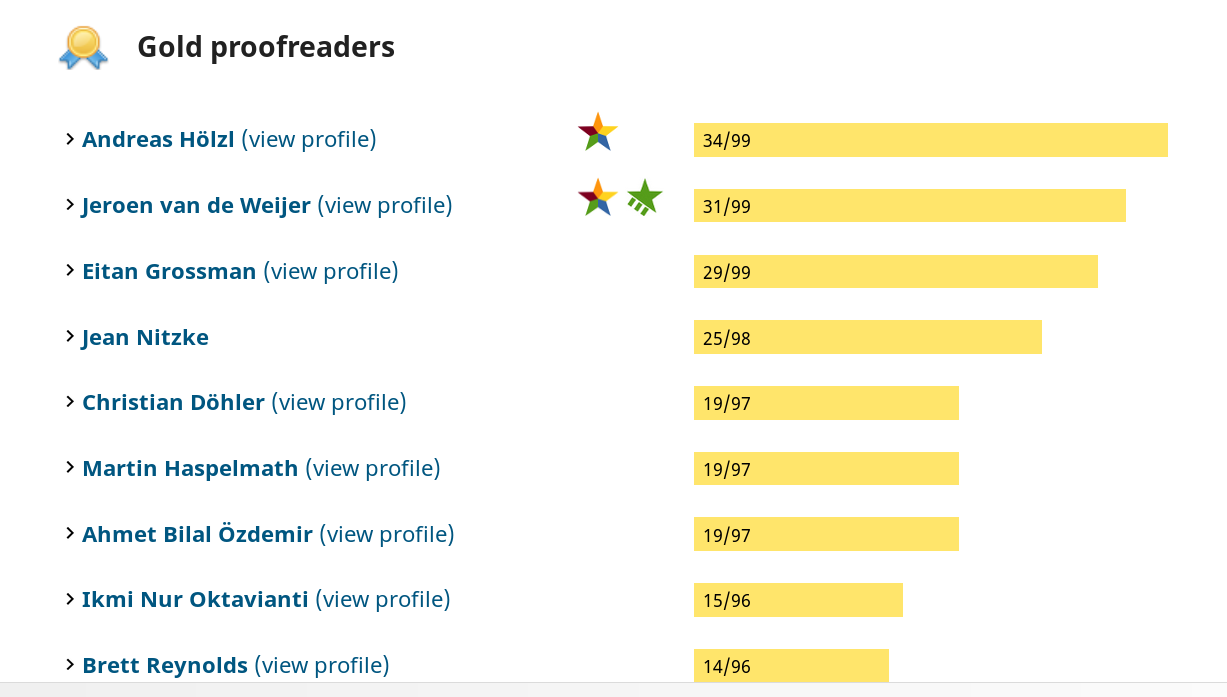
\includegraphics[height=\textheight]{halloffame.png}
}
\end{document}
